%%%%%%%%%%%%%%%%%%%%%%%%%%%%%%%%
\newpage
%%%%%%%%%%%%%%%%%%%%%%%%%%%%%%%%
\section{(C19,C20,C21,C22) Non-homogeneous equations: Method of undetermined coefficients}

\subsection*{Resources}
\begin{itemize}
    \item Video: All 4 Khan Academy videos starting at \url{https://www.khanacademy.org/math/differential-equations/second-order-differential-equations/undetermined-coefficients/v/undetermined-coefficients-1}
\end{itemize}

\subsection*{Comment}
The 2nd-order equations we were considering until now were homogeneous equations (ie, the RHS was zero). We can now build upon this to expand our ability to solve non-homogeneous equations (ie, where the RHS of the equation is non-zero).

The Khan Academy videos give an excellent initial introduction to the subject, and so please do take the time to view and take notes about all four videos in the series.

In the 4th video Mr Kahn describes about how it is possible to add solutions if there are multiple terms on the right. This occasionally causes confusion. Consider for example:

\begin{equation}
    y'' - 3y' - 4y = 2 \sin x
\end{equation}

This corresponds to the particular solution

\begin{equation}
    y_p = A \sin x + B \cos x
\end{equation}

A common point of confusion is about what to do in the case of something like
\begin{equation}
    \label{eq:particularconfusion}
    y'' - 3y' - 4y = 2 \sin x + 2 \cos x
\end{equation}

Should you just write $y_p = (A \sin x + B \cos x) + (C \sin x + D \cos x)$? After all, you have two terms in equation \ref{eq:particularconfusion} (ie, $2 \sin x$ and $2 \cos x$). You can note however that $A \sin x + C \sin x$ simplifies to $E \sin x$ where $E$ is just another constant (in this case $A+B$) so in the end you will be left with $y_p = E \sin x + F \cos x$. So while it may be clearer to explicitly calculate coefficients for every term on the RHS, in many cases the terms will simplify.


\subsection*{Challenge}
Find the general solution of the following non-homogeneous differential equations:

1. (C19) $y'' + 4y = 8$\\
2. (C20) $y'' + 4y = 8t^2 - 20t + 8$\\
3. (C21) $y'' + 4y = 5 \sin 3t - 5 \cos 3t$\\
4. (C22) $y'' + 4y = 24 e^{-2t}$

(please just rate the challenges on challenge-hub after you have determined the answer for each one)

\subsection*{Solution}
The solutions are contained in the list on the next page in no particular order. Your answers should match one of the solutions given. Please try to not look at the solutions before completing the questions, since this will facilitate deep understanding and reproduce a real-life/exam environment.
\newpage
$y = C_1 \cos 2t + C_2 \sin 2t + 3e^{-2t}$\\ %4
$y = C_1 \cos 2t + C_2 \sin 2t + 8e^{-2t}$\\
$y = C_1 \cos 2t + C_2 \sin 2t + 2t^2 - 5t + 1$\\ %2
$y = C_1 \cos 2t + C_2 \sin 2t + 3t^2 + t + 3$\\
$y = C_1 \cos 2t + C_2 \sin 2t + \cos 3t - \sin 3t$\\ %3
$y = C_1 \cos 2t + C_2 \sin 2t + 2$\\ %1
$y = C_1 \cos 2t + C_2 \sin 2t + 5$\\



%%%%%%%%%%%%%%%%%%%%%%%%%%%%%%%%
\newpage
%%%%%%%%%%%%%%%%%%%%%%%%%%%%%%%%
\section{(C23-28) Method of undetermined coefficients II}

\subsection*{Comment}
The following pages go into more detail than the videos, considering a greater range of cases. You may note that here the particular solution is denoted by $Y$ while Sal Khan denoted it as $y_p$ in the videos.

\emph{The following notes were developed by Zachary S. Tseng at Pennsylvania State University, USA (\url{http://www.math.psu.edu/tseng/}). Included here with kind permission.}

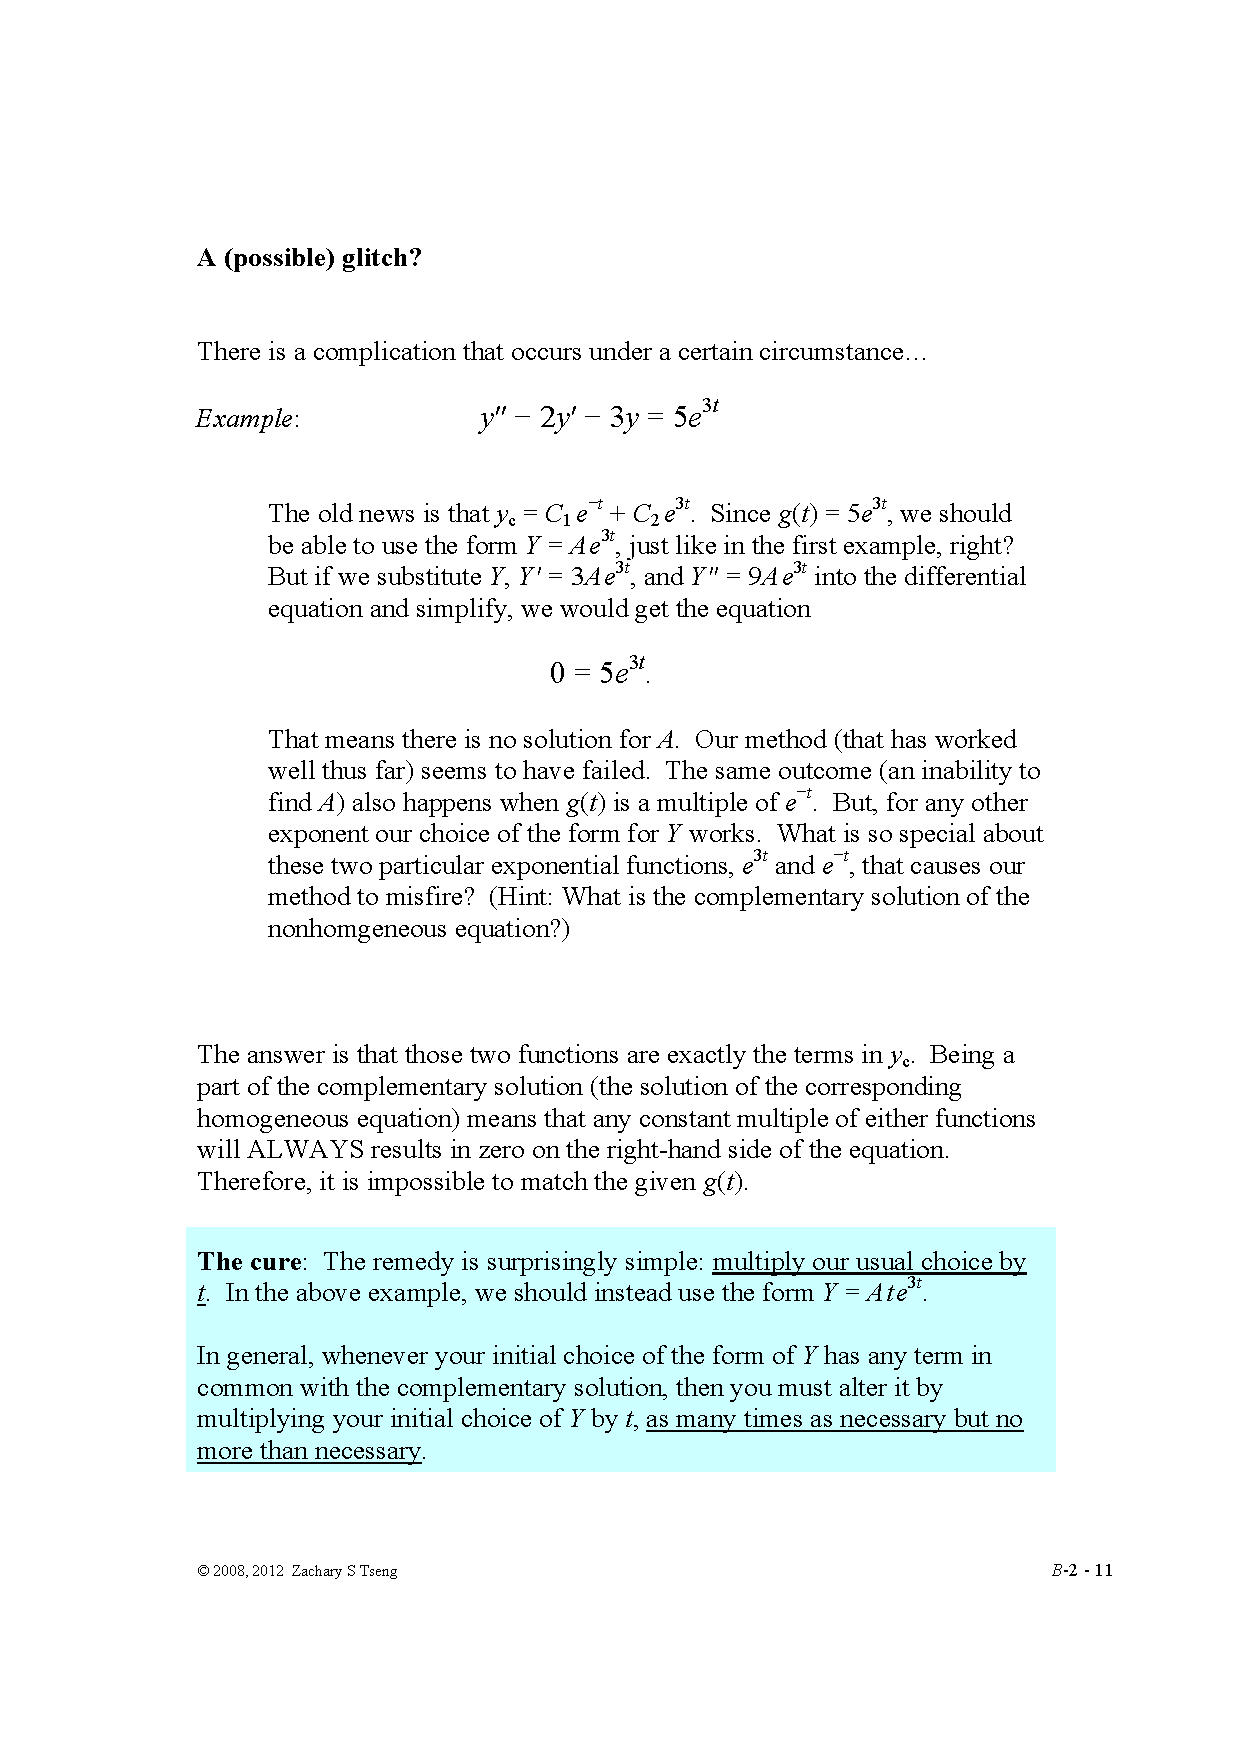
\includepdf[pages=-,pagecommand={},width=\textwidth,nup=1x1,frame=true]{External/undetermined.pdf}

\subsection*{Challenge}
The following challenges expand the range of problems to give you practise in a range of situations.

1. (C23) $y'' + 4y = 8 \cos 2t$\\
2. (C24) $y'' + 2y' = 2 te^{-t}$\\
3. (C25) $y'' + 2y' = 6 e^{-2t}$\\
4. (C26) $y'' + 2y' = 12 t^2$\\
5. (C27) $y'' - 6y' - 7y = 13 \cos 2t + 34 \sin 2t$\\
6. (C28) $y'' - 6y' - 7y = 8e^{-t} - 7t - 6$

\subsection*{Solution}
Assuming that the constants you find in your solution are all equal to 1, check your answer by calculating $y(t=0.4)$ in each case. To check your answer, please subsume all constants on any term into the constant that you set to 1. For example, instead of $y(t) = -2 C_1 e^{-t} + e^{-t}$, write $y(t) = C_1 e^{-t}$ where the two $e^{-t}$ terms have been combined and the $-2$ has been subsumed into the constant $C_1$, and then set $C_1 = 1$ to check the answer.




%%%%%%%%%%%%%%%%%%%%%%%%%%%%%%%%
\newpage
%%%%%%%%%%%%%%%%%%%%%%%%%%%%%%%%
\section{(C29) Method of undetermined coefficients: Determining the ODE I}

\subsection*{Comment}
This challenge gives you useful practise of going the other way; determining a differential equation that describes a given solution.

\subsection*{Challenge}
Determine the 2nd-order linear differential equation which has the general solution
\begin{equation}
    y = C_1 \cos 4t + C_2 \sin 4t - e^t \sin 2t
\end{equation}

\subsection*{Solution}
You will end up with differential terms on the left side and a function of $t$ on the right side.
Please compare your answer with your partner in class.
To check your answer with challenge-hub, evaluate the right side of your equation by substituting the value $t=0.4$.




%%%%%%%%%%%%%%%%%%%%%%%%%%%%%%%%
\newpage
%%%%%%%%%%%%%%%%%%%%%%%%%%%%%%%%
\section{(C30) Method of undetermined coefficients: Determining the ODE II}

\subsection*{Comment}
This challenge gives you useful practise of going the other way; determining a differential equation that describes a given solution.

\subsection*{Challenge}
Determine the 2nd-order linear differential equation which has the general solution
\begin{equation}
    y = C_1 e^{-2t} + C_2 t e^{-2t} + t^3 - 3t
\end{equation}

\subsection*{Solution}
You will end up with differential terms on the left side and a function of $t$ on the right side.
Please compare your answer with your partner in class.
To check your answer with challenge-hub, evaluate the right side of your equation by substituting the value $t=0.4$.
